\chapter{A Static Scheduling Language for Parallel Tree Traversals}
\label{chap:3}

We now introduce a static scheduling language for parallel computations over a tree such as those seen in layout. A compiler takes an attribute grammar (the functional specification) and its schedule and outputs an implement, i.e., a layout engine. For now, we ignore the source of the schedule. Beyond presenting the language and compilation strategy, we show how to verify functional and behavioral (parallel) correctness, introduce the first parallel schedule for a large subset of CSS, and show how, on GPU tree computations, memory may be dynamically allocated quite efficiently.

The goal of our language for traversals over trees is to benefit from high-performance computing techniques  commonly used for stencils over grids. Common for physical modeling, a stencil computation is one where a kernel only reads and writes to a limited set of nodes, there are many kernels, and the data dependencies between kernels lead to traversal patterns such as a wavefront. Many variants of stencils exist. The enthusiasm for them stems from programmers or stencil compilers being able to exploit knowledge of their structure to effectively optimize for use of cache lines, memory, parallel processors, and other resources. Similar techniques are known for trees, and the next chapter introduces additional ones.

Our first challenge in this chapter is to restrict the scheduling language enough to facilitate optimization while still providing the flexibility for expressing  document layout and data visualization workloads. Finding parallelism in CSS is already novel,  so being further able to optimize it with techniques associated with small formulas for physical models is surprising. We found that, while layout computations have too many data dependencies to be solved with one simple tree traversal, sequences of 3--5 traversals often suffice for data visualizations and 9 for CSS. Our scheduling language therefore consists of traversal patterns, such as parallel top down (\emph{preorder}) traversal of the tree, and ways of combining them, such as in a sequence. One especially representative case study of matching restrictions with flexibility was in our study of  visualizations: dynamic memory allocation on a GPU is generally a bottleneck, but we used a sequence of tree traversals for parallel allocation of render buffers for each node.

Another artifact of layout specifications being magnitudes bigger than stencil formulas is that the correctness concerns change. For stencil computations, the verification challenge lies more in correctly optimizing the implementation of a traversal schedule. Layout computations encounter a challenge before that point: the size of the functional specification and the ensuing tangle of data dependencies require ensuring  that the parallel schedule itself is safe to implement. We use a variant of existing static dependency analyses of attribute grammars to verify that the schedule is race-free. 

Our use of static analysis for the attribute grammars leads to an important result for layout languages: we show how to statically verify three important properties about them.  
\begin{itemize}
\item \textbf{Totality} The layout language defines a solution for every syntactically well-formed input tree; it is unambiguous. 
\item \textbf{Determinism} As discussed  in the previous paragraph, parallelization is safe.
\item \textbf{Linearity (Single Assignment)} Every attribute is assigned to exactly once. Layout languages often perform \emph{reflow} to iteratively solve constraints or incremental computation, so this property bounds the need for it. 
\end{itemize}
The first property demonstrates the ability to reason about \emph{functional correctness} and the last two about \emph{behavioral correctness}. Put together, we verify that a language is unambiguous, supports parallelization, and with bounded asymptotic complexity. 


\section{Language of Static Schedules}
%Our approach builds upon the ideas of multipass attribute grammars and statically ordered attribute grammars~\cite{oag}. Before showing our technique, we review how to use these ideas on how to more efficiently evaluate attribute grammars than the na\"{i}ve dynamic approach of Chapter~\ref{chap:2}. Furthermore, we review how they enable proving properties about the attribute grammars such as unambiguity, and (inefficient) parallelization strategies. 

This section focuses on defining our full language of traversal schedules. It is the input for our code generators. Programmers either do not specify the schedule in practice due to our automation support, or use the \emph{sketching} extension (Section~\ref{sec:holes}) for more succinct partial specification.

Statically scheduled evaluation departs from the dynamic evaluation strategy of Chapter~\ref{chap:2}. Static scheduling solves the performance problem of dynamic evaluation repeatedly manipulating the data dependencies of every attribute at runtime. For example, what would be a direct sequence of arithmetic statements in a static language becomes an interleaving of graph manipulations and arithmetic with the dynamic evaluator. The runtime scheduling overhead for evaluating all the statement is (at least) linear in the size of the data dependency graph. 

Instead, a schedule statically specifies most of the scheduling decisions.  It specifies a sequence of tree traversals and the order of statements to use within each traversal. During a traversal at runtime, the order of nodes to traverse is based on the traversal pattern, such as top-down, rather than by inspecting data dependencies. Likewise, the statements to execute for a node are looked up based on the node's type rather than by data dependencies.  Our approach is a more compositional variant of others. Our flexibility requirements led to focusing on the ability to compose different types of traversals, such as by sequencing and nesting.






\newsavebox{\seqtraversals}
\begin{lrbox}{\seqtraversals}% Store first listing
\begin{minipage}{1\columnwidth}
\begin{lstlisting}[mathescape,language=C++,morekeywords={spawn,join}]
void preorder(void (*visit)(Prod &), Prod &p) {
  visit(p);
  for (Prod rhs in p) 
    parPre(visit, rhs);
}
void postorder(void (*visit)(Prod &), Prod &p) {
  for (Prod rhs in p) 
    parPost(visit, rhs);
  visit(p);
}
\end{lstlisting}
\end{minipage}
\end{lrbox}

\newsavebox{\seqtraversalsequence}
\begin{lrbox}{\seqtraversalsequence}% Store first listing
\begin{minipage}{1\columnwidth}
\begin{lstlisting}[mathescape,language=C++,morekeywords={spawn,join}]
postorder(visit1, start); 
preorder(visit2, start);
\end{lstlisting}
\end{minipage}
\end{lrbox}


\newsavebox{\hboxvisitors}
\begin{lrbox}{\hboxvisitors}% Store first listing
\begin{minipage}{1\columnwidth}
\begin{lstlisting}[mathescape,language=C++]
void visit1 (Prod &p) {
  switch (p.type) {
    case S $\rightarrow$ HBOX:  break;
    case HBOX $\rightarrow$ $\epsilon$:
      HBOX.w = input(); HBOX.h = input(); break;
    case HBOX $\rightarrow$ HBOX$_1$ HBOX$_2$:
      HBOX$_0$.w = HBOX$_1$.w + HBOX$_2$.w;
      HBOX$_0$.h = MAX(HBOX$_1$.h, HBOX$_2$.h);
      break;
  }
}
void visit2 (Prod &p) {
  switch (p.type) {
    case S $\rightarrow$ HBOX:
      HBOX.x = input(); HBOX.y = input(); break;
    case HBOX $\rightarrow$ $\epsilon$: break;
    case HBOX $\rightarrow$ HBOX$_1$ HBOX$_2$:
      HBOX$_1$.x = HBOX$_0$.x;
      HBOX$_2$.x = HBOX$_0$.x + HBOX$_1$.w;
      HBOX$_1$.y = HBOX$_0$.y;
      HBOX$_2$.y = HBOX$_0$.y;
      break;
  }
}
\end{lstlisting}
\end{minipage}
\end{lrbox}




\begin{figure}
\subfloat[\textbf{Sequential sequence of traversals}]{\label{fig:hboxseq:sequence} \usebox{\seqtraversalsequence} } \\
\subfloat[\textbf{Two sequential traversal pattern}]{\label{fig:hboxseq:traversals} \usebox{\seqtraversals} } \\
\subfloat[\textbf{Scheduled and compiled visits for ~\hlang{}.}]{\label{fig:hboxseq:compiled} \usebox{\hboxvisitors} } \\
\caption{\textbf{Sequentially scheduled and compiled layout engine for \hlang{}.}}
\label{fig:hboxseq}
\end{figure}





\subsection{Specifying Sequential Schedules}  
We start by examining how to specify a safe static schedule for \hlang that respects any possible dynamic dependencies (Figure~\ref{fig:deps:full}).
%Research into statically scheduled sequential attribute grammars revealed a variety of scheduling options. For example, some computations can be solved in one traversal over a tree and therefore merged into a parser, while others require multiple traversals. We focus on several important options and the automated reasoning supported for them.

Figure~\ref{fig:hboxseq} shows a sequential implementation of \hlang decomposed into several pieces. The layout engine solves an input tree over a sequence of two traversals (Figure~\ref{fig:hboxseq:sequence}). The first traverses the tree in postorder, meaning from the leaves up to the root (''bottom-up'') and the second performs are preorder traversal, meaning from the root down to the leaves (''top-down''). Figure~\ref{fig:hboxseq:traversals} provides a sample implementation of generic traversal code. During a during traversal, each node is \emph{visited} exactly once in order to compute the attributes whose dependencies have been satisfied. Figure~\ref{fig:hboxseq:compiled} shows that the first pass computes widths and heights and the second pass computes the x and y positions.

The example follows a static schedule rather than manipulating a dynamic data dependency graph. The sequence of traversal invocations and the code used for the different cases for each traversal's visitor determine the schedule. Each traversal now only performs dynamic scheduling in the sense of maintaining a stack for recurring down the tree, which is a cost proportional to the number of nodes rather than the size of the dynamic dependency graph between attributes. In practice (Chapter~\ref{chap:6}), our compiler and runtime optimizations even eliminate the example's implicit use of a call stack.


The decompose the schedule into several types of policy fragments. First, the schedules involves a \emph{sequence} of  \emph{two different types} of traversals:
\begin{lstlisting}
      postorder(visit1, start); preorder(visit2, start)
\end{lstlisting}
Just one bottom-up traversal cannot compute all the attributes, such as all the x and y attributes that flow downwards (Figure~\ref{fig:deps:full}), so the schedule may require multiple types of traversals and in a careful order.  Furthermore, within a traversal, the schedule specifies different orders of statements for different types of nodes. Consider the following fragment:
\begin{lstlisting}
      HBOX$_1$.x = HBOX$_0$.x;
      HBOX$_2$.x = HBOX$_0$.x + HBOX$_1$.w;
\end{lstlisting}
The schedule specifies that \code{HBOX}$_2$\code{.x} can (and should) be immediately evaluated after \code{HBOX}$_1$\code{.x} without fear of unsatisfied data dependencies for any of its right-hand side terms. In summary, we see three parts to a schedule: the staging of traversals, the node visit order for every individual traversal, and the statement order for different types of nodes within a specific traversal.

We abstracted the three aspects of a schedule into a scheduling language (Figure~\ref{fig:hboxparallel}). For example, the schedule for the above computation would be appear as:
\begin{lstlisting}[mathescape,morekeywords={preorder,postorder}]
postorder
  HBOX$_0$ $\rightarrow$ HBOX$_1$ HBOX$_2$ { HBOX$_0$.w HBOX$_0$.h }
  HBOX $\rightarrow$ $\epsilon$ { HBOX.w HBOX.h }
;
preorder
  S $\rightarrow$ HBOX { HBOX.x HBOX.y }
  HBOX$_0$ $\rightarrow$ HBOX$_1$ HBOX$_2$ 
    { HBOX$_1$.x HBOX$_2$.x HBOX$_1$.y HBOX$_2$.y }
\end{lstlisting}
It specifies a sequence ('';'') of two traversals of node visit order \code{postorder} and \code{preorder}. For each type of node visited within a traversal, the schedule specifies the sequential sequence of attributes to evaluate. We note that, due to the desugaring of our class system in Section~\ref{sec:desugaring}, the dispatches in the above examples are based on grammar productions in the desugared representation. In terms of the fronted language, the dispatches are based on node class.

Generally, a single attribute grammar may be schedule in many ways. For example, the width and height computations share no dependencies, so the first postorder traversal might be partitioned into two postorder traversals:
\begin{lstlisting}[mathescape,morekeywords={preorder,postorder}]
postorder
  HBOX$_0$ $\rightarrow$ HBOX$_1$ HBOX$_2$ { HBOX$_0$.w }
  HBOX $\rightarrow$ $\epsilon$ { HBOX.w }
;
postorder
  HBOX$_0$ $\rightarrow$ HBOX$_1$ HBOX$_2$ { HBOX$_0$.h }
  HBOX $\rightarrow$ $\epsilon$ { HBOX.h }
;
preorder
  S $\rightarrow$ HBOX { HBOX.x HBOX.y }
  HBOX$_0$ $\rightarrow$ HBOX$_1$ HBOX$_2$ 
    { HBOX$_1$.x HBOX$_2$.x HBOX$_1$.y HBOX$_2$.y }
\end{lstlisting}
Rescheduling in this way may improve performance on small devices with little memory because the schedule cuts the working set size in half for each traversal. Note, however, that the schedule only optimizes execution; it does not change the result of evaluation.

\subsection{Compilation}
Compilation only requires an attribute grammar and the schedule. The traversal staging \code{postorder _ ; preorder _} directly translates to the executable fragment in Figure~\ref{fig:hboxseq:sequence}. Likewise, the mapping from traversal productions to statement sequences, such as \code{HBOX} $\rightarrow \epsilon$ \{ \code{HBOX.w HBOX.h} \}, directly translate to the visit functions of Figure~\ref{fig:hboxseq:compiled}. The translation matches an attribute in the schedule with the lefthand side attribute of an equation in the attribute grammar and outputs the full assignment statement in its place. 

Our code generation pipeline is further complicated but conceptually similar. The schedule is combined with the attribute grammar to form an intermediate representation, and different code generators target different backends, such as JavaScript, OpenCL, and C++. Furthermore, some of the reductions of Section~\ref{sec:desguaring} require augmenting or rewriting the intermediate representation, such as reinserting loops that were unrolled during scheduling (Section~\ref{???}). Our end-to-end compiler design is slightly different due to the synthesis algorithm (Chapter~\ref{chap:4})  and schedule autotuning (Section~\ref{sec:schedtuning}), but code generation for a schedule follows a more conventional process.


\newsavebox{\decomplang}
\begin{lrbox}{\decomplang}% Store first listing
\begin{minipage}{1\columnwidth}
\renewcommand{\litleft}{\bfseries}
\renewcommand{\ulitleft}{\bfseries}
\renewcommand{\superscript}[1]{\ensuremath{^{\textrm{#1}}}}
\renewcommand{\subscript}[1]{\ensuremath{_{\textrm{\uppercase{#1}}}}}
\renewcommand{\syntleft}{\normalfont\itshape}
\renewcommand{\syntright}{}
\begin{grammar}
<Sched> \deriv{} \emph{Sched} ; \emph{Sched}  ~ | ~ \emph{Sched} $\vert\vert$ \emph{Sched}  ~|~ \emph{Trav}

<Trav> \deriv{} <TravAtomic> \emph{Visit}*\{(<TravAtomic> $\mapsto$ \emph{Visit}*)*\}?

<TravAtomic>  \deriv{} "preorder" ~ | ~ "postorder" ~ | ~ "parPre"  ~ | ~  "parPost"  ~ | ~  "recursive" ~ 

<Visit> \deriv{} <Prod>  \{ \emph{Step}* \}

<Step> \deriv{} \emph{Attrib} ~ | ~ "recur" \emph{V} 
\end{grammar}
%<Sched, Trav, Visit, Step> \deriv{} \ldots ~ | ~ $\hole$        
\end{minipage}
\end{lrbox}


\newsavebox{\hboxdecomp}
\begin{lrbox}{\hboxdecomp}% Store first listing
\begin{minipage}{1\columnwidth}
\begin{lstlisting}[mathescape,morekeywords={parPre,parPost}]
parPost
  HBOX$_0$ $\rightarrow$ HBOX$_1$ HBOX$_2$ { HBOX$_0$.w HBOX$_0$.h }
  HBOX $\rightarrow$ $\epsilon$ { HBOX.w HBOX.h }
;
parPre
  S $\rightarrow$ HBOX { HBOX.x HBOX.y }
  HBOX$_0$ $\rightarrow$ HBOX$_1$ HBOX$_2$ 
    { HBOX$_1$.x HBOX$_2$.x HBOX$_1$.y HBOX$_2$.y }
\end{lstlisting}
\end{minipage}
\end{lrbox}

\newsavebox{\traversals}
\begin{lrbox}{\traversals}% Store first listing
\begin{minipage}{1\columnwidth}
\begin{lstlisting}[mathescape,language=C++,morekeywords={spawn,join}]
void parPre(void (*visit)(Prod &), Prod &p) {
  visit(p);
  for (Prod rhs in p) 
    spawn parPre(visit, rhs);
  join;
}
void parPost(void (*visit)(Prod &), Prod &p) {
  for (Prod rhs in p) 
    spawn parPost(visit, rhs);
  join;
  visit(p);
}
\end{lstlisting}
\end{minipage}
\end{lrbox}

\newsavebox{\hboxparvisitors}
\begin{lrbox}{\hboxparvisitors}% Store first listing
\begin{minipage}{1\columnwidth}
\begin{lstlisting}[mathescape,language=C++]
parPost(visit1, start); parPre(visit2, start);
\end{lstlisting}
\end{minipage}
\end{lrbox}


\begin{figure}
\subfloat[\textbf{One explicit parallel schedule for ~\hlang{}.}]{\label{fig:hboxparallel:schedule} \usebox{\hboxdecomp} } \\
\subfloat[\textbf{Na\"{\i}ve traversal implementations} with Cilk's~\cite{cilk} \sched{spawn} and \sched{join}.]{\label{fig:hboxparallel:traversals} \usebox{\traversals} } \\
\subfloat[\textbf{Scheduled and compiled layout engine for ~\hlang{}.}]{\label{fig:hboxparallel:compiled} \usebox{\hboxparvisitors} } \\
\subfloat[\textbf{Language of schedules} (without holes) ]{\label{fig:hboxparallel:decomplang} \usebox{\decomplang} }
\caption{\textbf{Scheduled and compiled layout engine for \hlang{}.}}
\label{fig:hboxparallel}
\end{figure}




\begin{figure}
\subfloat[First traversal: parallel postorder]{\label{fig:depsparallel:postorder}
\begin{minipage}{0.5\columnwidth}\centering
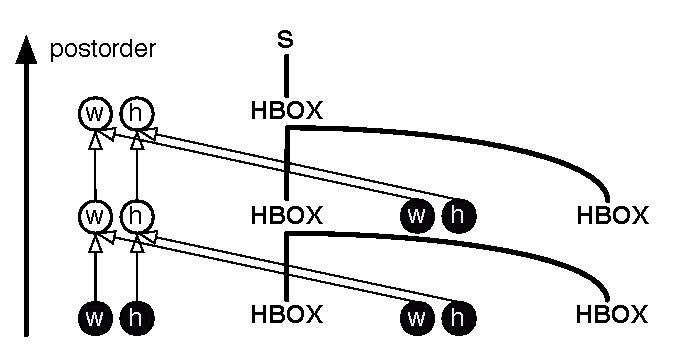
\includegraphics[trim=0 0 0 0,clip,width=1.0\columnwidth]{chapter3/depspostorder}
\end{minipage}}
\subfloat[Second traversal: parallel preorder.]{\label{fig:depsparallel:preorder}
\begin{minipage}{0.5\columnwidth}\centering
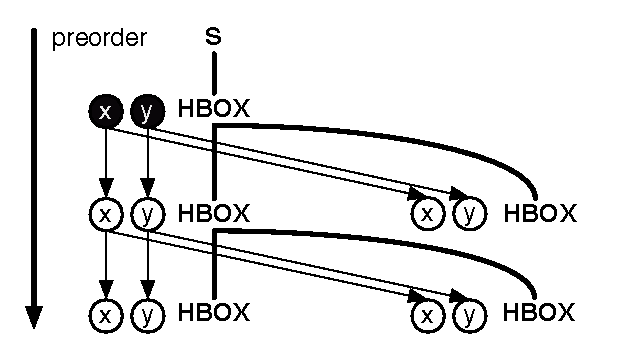
\includegraphics[trim=0 0 0 0,clip,width=1.0\columnwidth]{chapter3/depspreorder}
\end{minipage}}
\caption{\textbf{Parallel Traversal}. Shown for constraint tree  in Figure~ZZZ~(a). Circles denote attributes, with black circles denoting attributes with resolved dependencies such as \sched{input()}s. Thin lines show data dependencies and thick lines show production derivations. First diagram shows dependencies followed by first traversal, and second for the following traversal.}
\label{fig:depsparallel}
\end{figure}


\subsection{Parallel Schedules}
A schedule exposes structured parallelism within a traversal and across them. 

For an example of parallelism within a traversal, the first postorder traversal for \hlang features latent parallelism. The widths and heights for one subtree can be computed independently of the widths and heights of another distinct subtree. Figure~\ref{fig:depsparallel:postorder} shows an example where different (logical) threads may compute on the leaf nodes and implicit barriers force a join at every intermediate node. Likewise, the second traversal (Figure~\ref{fig:depsparallel:preorder}) may be changed to a parallel preorder traversal where ever intermediate node acts as a logical fork. Figure~\ref{fig:hboxparallel:traversals} depicts na\"{i}ve parallel implementations using Cilk's~\cite{??} \code{spawn} and \code{join} primitives. We formulate the schedule by changing the specification from \code{postorder} and \code{preorder} to \code{parPost} and \code{parPre} (Figure~\ref{fig:hboxparallel:schedule}).

We may exploit parallelism across traversals as well. For example, just as we created a different but functionally equivalent sequential schedule for \hlang, we can do the same manipulation to yield a new parallel schedule:
\begin{minipage}{1\columnwidth}
\begin{lstlisting}[mathescape,morekeywords={parPre,parPost}]
(   parPost
     HBOX$_0$ $\rightarrow$ HBOX$_1$ HBOX$_2$ { HBOX$_0$.w }
     HBOX $\rightarrow$ $\epsilon$ { HBOX.w }  
   $||$  
    parPost
     HBOX$_0$ $\rightarrow$ HBOX$_1$ HBOX$_2$ { HBOX$_0$.h }
     HBOX $\rightarrow$ $\epsilon$ { HBOX.h })
; parPre $\ldots$ $\emph{/* same as before */}$
\end{lstlisting}
\end{minipage}
The ``\|\|'' construct specifies that one traversal may be run concurrently with another. Neither traversal traversal depends on attributes written by the other, so the parallelizaton is safe. Even if we cannot exploit parallelism within a traversal, using ''\|\|'' enables us to exploit parallel across them. 


\section{Structured Parallelism in Visitors} 
\subsection{td, bu, in order} (related to distributed?)
\subsection{concurrent} (old paper: unstructured within visit)
\subsection{multipass} (any old paper? unstructured within visit)
\subsection{nested}


\section{Schedule Compilation}
Phrase as rewrites working in an EDSL w/ templates
\subsection{Rewrite rules}
\section{Schedule Verification}
\subsection{Overview}
\begin{itemize}
\item properties to prove: schedule followed (and complete), dependencies realizable 
\item structure of proof
\end{itemize}
\subsection{Axioms}
\begin{itemize}
\item axioms
\item examples from each
\end{itemize}
\subsection{Proof}

\section{Automatically Staging Memory Allocation for SIMD Rendering}
\newsavebox{\stagedAllocFull}
\begin{lrbox}{\stagedAllocFull}% Store first listing
\begin{lstlisting}[mathescape]
float *drawCircle (float x, float y, float radius) {
  float *buffer = malloc( (2 * sizeof(float) ) * round(radius))
  for (int i = 0; i < round(radius); i++) {
    buffer[2 * i] = x + cos(i * PI/radius);
    buffer[2 * i + i] = y + sin(i * PI/radius);
  }
  return buffer;
}
\end{lstlisting}
\end{lrbox}

\newsavebox{\stagedAllocAlloc}
\begin{lrbox}{\stagedAllocAlloc}% Store first listing
\begin{lstlisting}[mathescape]
int allocCircle (float x, float y, float radius) {
  return round(radius);
}
\end{lstlisting}
\end{lrbox}


\newsavebox{\stagedAllocRender}
\begin{lrbox}{\stagedAllocRender}% Store first listing
\begin{lstlisting}[mathescape]
int fillCircle(float x, float y, float radius, float *buffer) {
  for (int i = 0; i < round(radius); i++) {
    buffer[2 * i] = x + cos(i * PI/radius);
    buffer[2 * i + i] = y + sin(i * PI/radius);
  }	
  return 0;
}
\end{lstlisting}
\end{lrbox}


\begin{figure}
\subfloat[\textbf{Na\i{v}e drawing primitive .}]{\label{fig:stagedalloc:original} \usebox{\stagedAllocFull} }  \\
\subfloat[\textbf{Allocation phase of drawing}.]{\label{fig:stagedalloc:alloc} \usebox{\stagedAllocAlloc} } \\
\subfloat[\textbf{Tessellation phase of drawing}.]{\label{fig:stagedalloc:use} \usebox{\stagedAllocRender} } 
\caption{\textbf{Partitioning of a library function that uses dynamic memory allocation into parallelizable stages.}}
\label{fig:stagedalloc}
\end{figure}


\newsavebox{\twocirclesOrig}
\begin{lrbox}{\twocirclesOrig}% Store first listing
\begin{lstlisting}[mathescape]
CBOX $\rightarrow$ BOX$_1$ BOX$_2$
{
  ...
  CBOX.render = 
    drawCircle(CBOX.x, CBOX.y, CBOX.radius)
      + drawCircle(CBOX.x + 10, CBOX.y + 10, CBOX.radius * 0.5);
}
\end{lstlisting}
\end{lrbox}

\newsavebox{\twocirclesExpanded}
\begin{lrbox}{\twocirclesExpanded}% Store first listing
\begin{lstlisting}[mathescape]
CBOX $\rightarrow$ BOX$_1$ BOX$_2$
{
  ...
  CBOX.sizeSelf = 
    allocCircle(CBOX.x, CBOX.y, CBOX.radius)
      + allocCircle(CBOX.x + 10, CBOX.y + 10, CBOX.radius * 0.5);
  CBOX.size = CBOX.sizeSelf +BOX$_1$.size + BOX$_2$.size;
  BOX$_1$.buffer = CBOX.buffer + CBOX.sizeSelf;
  BOX$_2$.buffer = BOX$_1$.buffer + BOX$_1$.size;
  CBOX.render = 
    fillCircle(CBOX.x, CBOX.y, CBOX.radius, CBOX.buffer)
      + fillCircle(CBOX.x + 10, CBOX.y + 10, CBOX.radius * 0.5,
            CBOX.buffer + allocCircle(CBOX.x, CBOX.y, CBOX.radius));
}
\end{lstlisting}
\end{lrbox}

\newsavebox{\twocirclesMacro}
\begin{lrbox}{\twocirclesMacro}% Store first listing
\begin{lstlisting}[mathescape]
CBOX $\rightarrow$ BOX$_1$ BOX$_2$
{
  ...
  CBOX.render = 
      @Circle(CBOX.x, CBOX.y, CBOX.radius)
      + @Circle(CBOX.x + 10, CBOX.y + 10, CBOX.radius * 0.5);
}
\end{lstlisting}
\end{lrbox}




\begin{figure}
\subfloat[\textbf{Call into inefficient library.}]{\label{fig:stagedallocClient:original} \usebox{\twocirclesOrig} }  \\
\subfloat[\textbf{Macro-expanded calls into staged library}.]{\label{fig:stagedallocClient:expanded} \usebox{\twocirclesExpanded} }  \\
\subfloat[\textbf{Sugared calls into staged library}.]{\label{fig:stagedallocClient:macro} \usebox{\twocirclesMacro} } 
\caption{\textbf{Use of dynamic memory allocation in a grammar for rendering two circles.}}
\label{fig:stagedallocClient}
\end{figure}

\begin{figure}
\centering
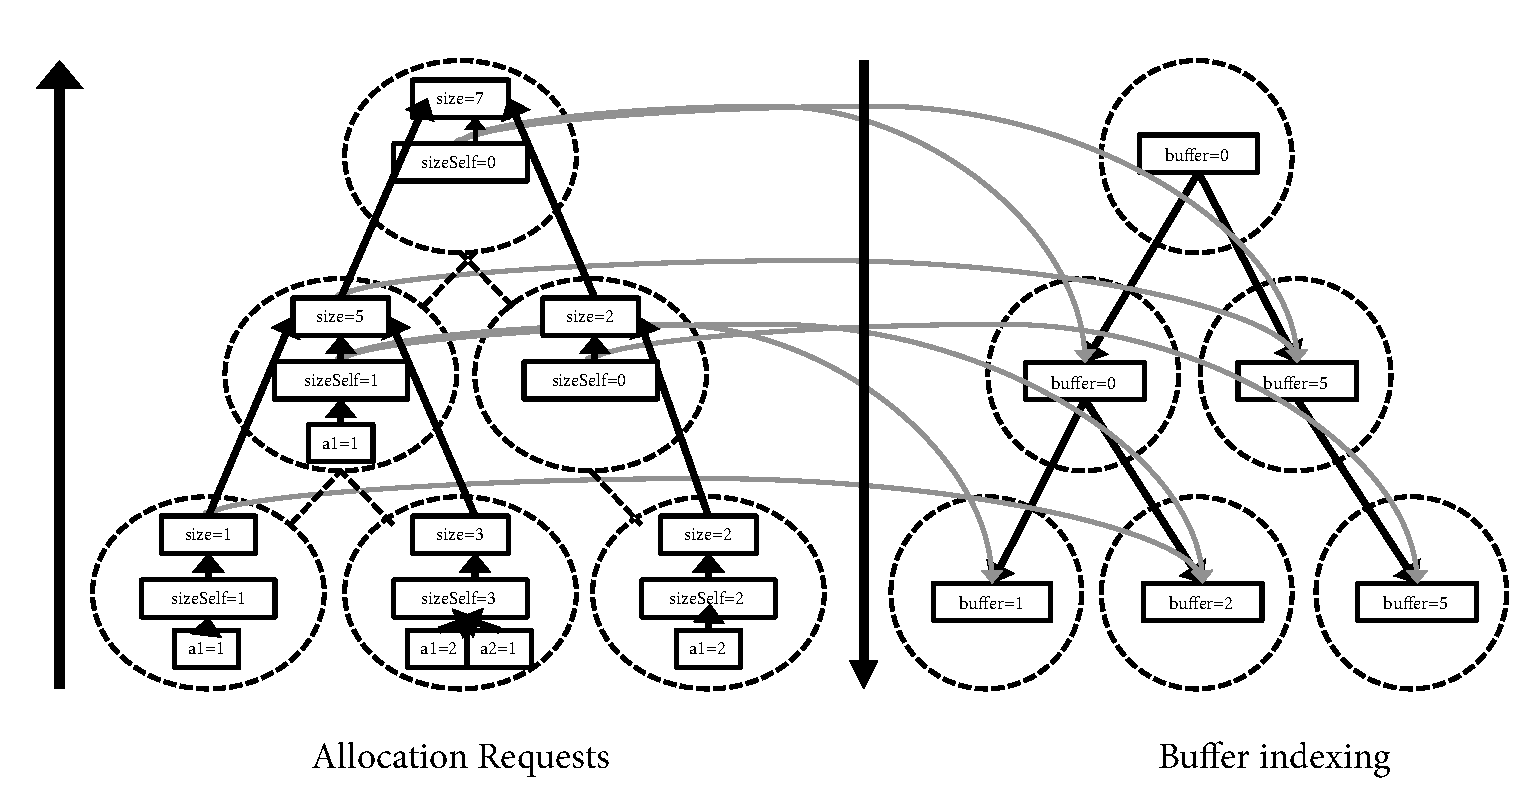
\includegraphics[trim=0 0 0 0,clip,width=1.0\columnwidth]{chapter6/macro}
\caption{\textbf{Staged parallel memory allocation as two tree traversals.} First pass is parallel bottom-up traversal computing the sum of allocation requests and the second pass is a parallel top-down traversal computing buffer indices. Lines with arrows indicate dynamic data dependencies.}
\label{fig:renderingtraversal}
\end{figure}


\subsection{Problem}
The static language of traversals is restricted, but we find that it can express important cases of typically more dynamic constructs. Prominent in our case studies, dynamic memory allocation provides significant flexibility for a language, but it is unclear how to perform it on a GPU without significant performance penalties. Our insight is that the memory allocation may be staged with parallel traversals by using a variant of prefix sum node labeling. One pass gathers  memory requests, a bulk allocation for the total amount is made, and then a scatter pass provides each node with a contiguous memory segment of it. We found manipulating memory addresses in this way to be error-prone, so we created two complementary automation techniques. First, we use our synthesizer to automatically schedule parallel memory allocation. Second, we syntactically hide the use of our optimization through a macro that automatically expands into staged dynamic memory allocation and consumption calls.

For example, we found parallel dynamic memory allocation to simplify the transition between layout and rendering. All nodes that render a circle will call some form of \code{drawCircle} in Figure~\ref{fig:stagedalloc:original}. Depending on the size of the circle, which is computed as part of the layout traversals, a different amount of memory will be allocated. Once the memory is allocated, vertices will be filled in with the correct position. The rendering engine will then connect the vertices with lines and paint them to the screen. The processing of converting the abstract shape into renderable vertices is known as tessellation. We want our system to tesselate the display objects for each node in parallel.




\subsection{Staged Parallel Memory Allocation}
We stage the use of dynamic memory into four logical phases: 
\begin{enumerate}
\item Parallel request (bottom-up tree traversal to gather )
\item Physical memory allocation
\item Parallel response (top-down tree traversal to scatter)
\item Computations that consume dynamic memory (normal parallel tree traversals)
\end{enumerate}
 The staging allows us to parallelize the request and response stages. We reuse the parallel tree traversals for them, as well as for the actual consumption. The actual allocation of physical memory in stage 2 is fast because it is a single call. Figure~\ref{fig:renderingtraversal} shows the dynamic data dependencies and two parallel tree traversals for an instance of staged parallel memory allocation.

Library functions that requires dynamic memory allocation are manually rewritten into allocation request  (Figure~\ref{fig:stagedalloc:alloc}) and memory consumption fragments (Figure~\ref{fig:stagedalloc:Render}). The transformation was not onerous to perform on our library primitives and, in the future, might be automated. 

Invocations of the original in the attribute grammar are rewritten to use the new primitives. For example, drawing two circles (Figure~\ref{fig:stagedallocClient:original}) is split into calls for allocation requests, buffer pointer manipulation, and buffer usage (Figure~\ref{fig:stagedallocClient:expanded}). The transformation increases memory consumption costs due to book keeping of allocation sizes. 

The result of our staging is three logical parallel passes, which, in practice, is merged into two parallel passes over the tree. The first pass is bottom up, similar to a prefix sum: each node computes its allocation requirements, adds that to the allocation requirements of its children,and then the process repeats for the next level of the tree. The \code{sizeSelf} and \emph{size} attributes are used for the first pass. Once the cumulative memory needs is computed, a bulk memory allocation occurs, and then a parallel top-down traversal assigns each node a memory span from \code{buffer} to \code{buffer + selfSize}. Finally, the memory can be used for actual computations through normal parallel passes. Memory use can occur immediately upon computation of the buffer index, so the last two logical stages are merged in implementation.

\subsection{Automation with Automatic Scheduling and Macros}
Manually manipulating the allocation requests and buffer pointers is error prone. We eliminated the problem through two automation techniques: automatic scheduling to enforce correct parallelization and macro expansion to encapsulate buffer manipulation.

To enforce proper parallelization, we relied upon our synthesizer to schedule the calls. If the synthesizer cannot schedule allocation calls and buffer propagation, it reports an error. Our insight is that, implicit to our staged representation, we could faithfully abstract the memory manipulations as foreign function calls. Our synthesizer simply performs its usual scheduling procedure.

To encapsulate buffer manipulation, we introduced the macro '@'.  Code that uses it is similar to code that assumes dynamic memory allocation primitives: the slight syntactic difference can be seen between Figure~\ref{fig:stagedallocClient:macro}  and Figure~\ref{fig:stagedallocClient:original}. Our macros (implemented in OMetaJS~[[CITE]]) automatically expand into the form seen in Figure~\ref{fig:stagedallocClient:expanded}. 

Our use case only required one allocation stage, but multiple may be needed.  For example, a final logging stage might be added that should run after all other computations, including rendering. However, the '@' calls described above expand to contribute to one attribute (\code{size}): no allocation is made until all of the sizes are known, which prevents making an allocation after using dynamic memory. To support multiple allocation stages, the '@' macro could be expanded to include logical group names: \code{@[render]Circle(...)} would contribute to \code{sizeRender}, \code{@[log]error(...)} to \code{sizeLog}, and \code{@[render,log]Strange(...)} to both \code{sizeRender} and \code{sizeLog}. Parallel traversals would be created for each logical name, and the synthesizer would be responsible for determining if the traversals can be merged in the final schedule and implementation.



\section{Scheduling Loops}


\section{Evaluation: Layout as Structured Parallel Visits}
\subsection{Box model}
\subsection{Nested text}
\subsection{Grids}


\subsection{SIMD Rendering through Staged Memory Allocation}
We evaluate three dimensions of our staged memory allocation approach: flexibility, productivity, and performance. First, it needs to be able to express the rendering tasks that we encounter in GPU data visualization. Second, it should some form of productivity benefit for these tasks. Finally, the performance on those tasks must be fast  enough to support real-time animations and interactions of big data sets.



\subsubsection{Productivity}
Productivity is difficult to measure. Before using the automation extensions for rendering, we repeatedly encountered bugs in manipulating the allocation calls and memory buffers. The bugs related both to incorrect scheduling and to incorrect pointer arithmetic. Our new design eliminates the possibility of both bugs.

One suggestive productivity measure is of how many lines of code the macro abstraction eliminates from our visualizations. We measured the impact on using it for 3 of our visualizations. The first visualization is our HBox language extended with rendering calls, while the other two are interactive reimplementations of popular visualizations: a treemap~[[CITE]] and multiple 3D line graphs~[[CITE]].


\begin{table}[ht]
\caption{Lines of Code Before/After Invoking the '@' Macro}
\centering
\begin{tabular}{c r r r}
\hline\hline
 \textbf{Visualization} & \textbf{Before (loc)} & \textbf{After (loc)} & \textbf{Decrease} \\ [0.5ex] \hline
  HBox & 97 & 54 & 44\% \\
  Treemap & 296 & 241 & 19\% \\
  GE & 337 & 269 & 20\% \\ [1ex] 
\hline
\end{tabular}
\label{table:macroreduction}
\end{table}
Table~\ref{table:macroreduction} compares the lines of code in visualizations before and after we added the macros. Using the macros eliminated 19--44\% of the code. Note that we are \emph{not} measuring the macro-expanded code, but code that a human wrote.



As shown in Figure~\ref{fig:stagedallocClient}, the eliminated code is code that was introduced by staging the library calls. Porting unstaged functional graphics calls to the library, is in practice, an alpha renaming of function names.  Using the '@' macro eliminates 19--44\% of the code that would have otherwise been introduced and completely eliminates two classes of bugs (scheduling and pointer arithmetic), so the productivity benefit is non-trivial. 

\subsubsection{Performance}


\section{Related Work}
Lang of schedules
\begin{itemize}
\item background
\item stencils and skeletons: wavefront, ...
\item polyhedra
\end{itemize}
Schedule verification
\begin{itemize}
\item compare to OAG etc., looser dataflow/functional langs
\end{itemize}